\chapter{Background}
\label{chapterlabel2}
In this chapter, background related to the physiology of the cardiovascular system and computational fluid dynamics in this field will be introduced. Additionally, the process of verification, validation and uncertainty quantification will be explained.


\section{Cardiovascular system}
The cardiovascular system, also called the circulatory system, is a closed-loop system composed by the heart, blood vessels and blood. It uses blood as the medium to distribute oxygen and nutrients to all body tissues and dispose of carbon-dioxide and metabolic waste to lungs and excretory organs. Additionally, the secondary function of the system is to redistribute bioactive agents and hormones throughout the body, and regulate the body temperature \cite{Levick2010Introduction5ed}.\par

The heart is a muscular organ that  pumps the blood into the blood vessels to distribute it around the body. It is located in between the lungs above the sternum. The heart is divided into two sides and each side is divided further into two chambers (as seen on Figure \ref{fig:heart}. The top chambers are the atria and the bottom ones are the ventricles. The wall of the heart are composed of cardiac muscle which produce contraction that pump the blood into the arteries \cite{aaronson2012cardiovascular,tortora2017introduction}. \par

The system is divided into two circulatory loops with the heart at the center, a pulmonary circulation and systemic circulation. In the pulmonary circulation, the deoxygenated blood is pumped from the heart's right ventricle into the pulmonary artery, where the blood is transported into the lungs where an oxygen exchange occurs. The blood then returns to the left atrium, passes through the left ventricle into the systematic circulation\cite{Levick2010Introduction5ed,tortora2017introduction}. \par


\begin{figure}[ht!]
  \centering
  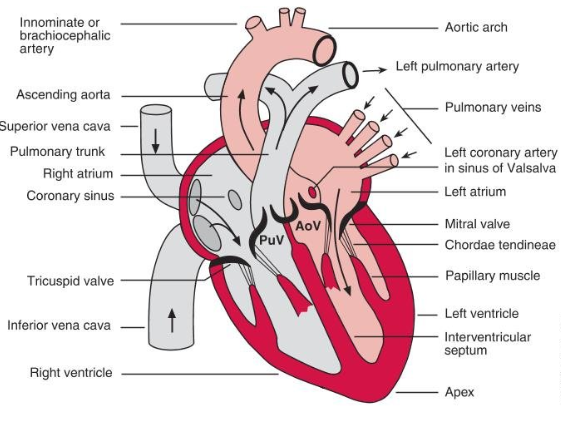
\includegraphics[width=0.6\textwidth]{Figures/heart.PNG}
  \caption{Structure of the heart and connection to the major veins and arteries \cite{Levick2010Introduction5ed}.}
  \label{fig:heart}
\end{figure}


Blood vessels in the system are responsible to deliver the blood into organs and tissue. The blood is driven into the aorta from there it flows into the major arteries, which then deliver blood to the major regions and organs. The arteries can further branch out and then they converge into veins which transport the blood back into the heart \cite{Levick2010Introduction5ed}.\par

\section{Computational Modelling for cardiovascular applications}
Computational models have been often used to study the haemodynamics of the a system. These have been often used for hypothesis creation, mechanistic understanding, device evaluation or educational purposes. With better imaging modalities and improved devices to obtain patient measurements, patient-specific modelling has emerged, showcasing their predictive power and their capability of being used in diagnosis or predictive medicine was considered. Where the models are made tailored to the patient anatomy.\par
\begin{figure}
    \centering
    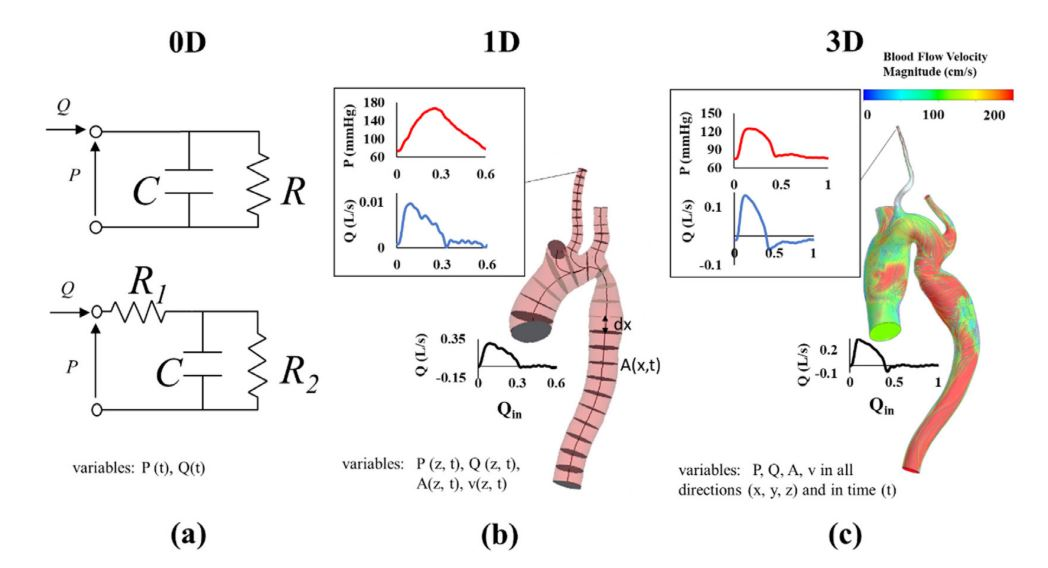
\includegraphics[width=\textwidth]{Figures/CardioMod.JPG}
    \caption{Illustration of \textbf{a)} zero-dimensional, \textbf{b)} one-dimensional and \textbf{c)} three dimensional vascular models \cite{Hose2019CardiovascularNext}}
    \label{fig:CardioMod}
\end{figure}

Cardiovascular models can be categorised by their dimension as seen on Figure \ref{fig:CardioMod}. Zero-dimensional (0D), or lumped parameter models, divide the system into individual components and represent effects through lumped parameters. The governing equations are ordinary differential equations. Lumped parameter models of the circulation are analogous to an electrical circuit where the physiological variables pressure, volume and flow are equivalent to to voltage, charge and current. 0D models can be used to simulate the global haemodynamic in the whole circulation system \cite{Zhou2019APressure} and can be extended to include biochemical and biomechanical processes \cite{Hose2019CardiovascularNext}. \par

One dimensional models (1D) are distributed parameter models, which can represent distributed properties along the vessel axis. These models are represented using partial differential equations in time and one spatial dimension and they are used to study pulse wave transmission \cite{Zhou2019APressure, Hose2019CardiovascularNext}. \par 

\subsection{Computational Fluid Dynamics}
A three-dimensional analysis of the flow in a patient-specific anatomy yields spatial and temporal on variables such as flow, pressure, wall shear stress or wall displacemet. The governing equations of the flow are the Navier-Stokes equations (\ref{eq:n_s}), which describe the conservation of momentum of a fluid.
% rewrite
Thus, the flow can be calculated in conjunction with the conservation of mass equation (\ref{eq:con} ):
\begin{equation}
\frac{\partial \rho}{\partial t}+\nabla \cdot (\rho U) = 0 \\
\label{eq:con}
\end{equation}
\begin{equation}
\frac{\partial (\rho U)}{\partial t}+\nabla \cdot (\rho U \times U) = -\nabla p + \nabla \cdot \tau + S_{M}
\label{eq:n_s}
\end{equation}
where, $p$ and $\tau$ are the pressure and stress tensor, respectively and $U$ is the velocity of the flow. The term $S_M$ refers to external forces to the system. \par

\subsection{Patient-specific data}
In order to create image-based patient-specific haemodynamics models, it is necessary to obtain geometry and flow data. \par

Imaging techniques such a computed tomography (CT) can be used to obtain a number of image slices which would then be used to reconstruct the 3D model of the tissue and organs of the patient. The method  uses ionising radiation which benefits from high spatial resolution and high penetration depth. However, CT scanning often has limited sensitivity and also exposes the patient to radiation \cite{Saremi2015CoronaryCT}. An alternative method to obtain the geometry can be magnetic resonance imaging (MRI) which uses the principles of electromagnetism to capture the images. It yields the images based on the radiofrequency of the tissue, generated by the hydrogen atoms within the tissues. Using MRI, the patient is not exposed to radiation or contrast agents. However, in comparison with the CT images, MRI has lower spatial resolution and is much more time-consuming to acquire whole 3D stack of images \cite{Maurovich-Horvat2012DifferentiationHearts, Karmonik2008ComputationalRates}.\par

Other patient-specific data such as volumetric flow, pressure  or wall displacement data has to be obtained in order to create accurate haemodynamic models. There are numerous ways how these can be obtained, both invasively and non-invasively. While invasive methods can provide accurate measurements through the application of different sensors, their application is restricted and use carefully considered. Several non-invasive imaging techniques can be employed. Doppler echocardiography or phase contrast (PC) MRI have shown to be a good method for obtaining flow measurements non-invasively \cite{Whitlock2015NoninvasiveAorta}. For wall, the time-resolved images must be obtained; this can be done using electrocardiogram (ECG) coupled with CT or 4D MRI data for example \cite{Bonfanti2017ComputationalData,Alimohammadi2015AorticUnderstanding}.

\subsection{Modelling assumptions}
Different modelling assumptions are used to explore computationally cardiovascular conditions. These will be briefly presented bellow.

\subsubsection{Boundary conditions}
Boundary conditions are essential in order to obtain realistic results.  \par

A number of inlet conditions can be imposed. The velocity profile can be considered either as uniform or as parabolic profile (Poiseuille or Womersley) \cite{Steinman2019HowVariability, Alimohammadi2015AorticUnderstanding}. If patient-specific data on the flow rates are absent, usually a necessary simplification is necessary where the flow rate is taken from previous studies or averaged from a published cohort. Another method would be scaling the waveform shape from literature by the vessel diameter \cite{Morris2016ComputationalMedicine}. \par

At the outlets, the simplest boundary condition to apply is constant pressure outlet (usually zero). This is usually done in rigid-wall simulation, where the pressure drop drives the flow rather then the absolute pressure. Another approach applies a scaling law to the outlet, where the pressure at the outlet could depend on the outlet's diameter or branch length which shows to have much superior estimation to the zero-pressure assumption \cite{Pirola2017OnDynamics, Les2010QuantificationDynamics}. \par

Most simulations assume the walls of the arteries to be rigid with a no-slip condition. However, as the arterial wall is compliant,  a number of studies suggest that the wall motion is an important factor that could influence the variables of interest \cite{Alimohammadi2017, Bonfanti2018AInteraction}. One of the method common method of modelling the wall displacement is using the fluid-structure interaction where the wall is modelled as an elastic wall where it expands with pressure changes. However, in comparison to the rigid wall simulation, this method is computationally expensive \cite{Steinman2012AssumptionsHemodynamics}.

\subsubsection{Blood viscosity model}
Blood is a complex fluid composed of red and white blood cells and platelets in plasma. While blood exhibits non-Newtonian properties, many of the haemodynamic models assume blood as a Newtonian fluid in large arteries. While the strain rates in these vessels are very low \cite{Fung1997BiomechanicsCirculation}, the Newtonian fluid does not take into account the shear-thinning properties of blood. By increasing the shear rate on the blood, the viscosity decreases (as seen in Figure \ref{fig:visc}) as a result of the disaggregation and the deformation of red blood cells \cite{Gijsen1999TheModel,Cho1991EffectsFlows}. Simple non-Newtonian models, such as Carreau-Yasuda or Casson, have been used to approximate the complex behaviour of the blood and to improve the study of the properties of the blood in vessels  \cite{Alimohammadi2015PredictingApproach}. \par

\begin{figure}[ht!]
\centering
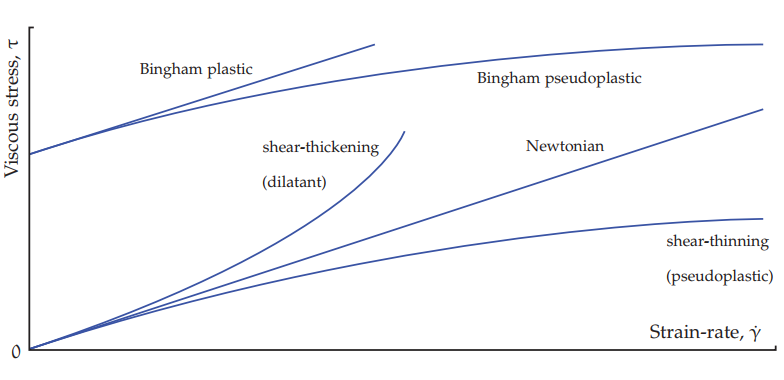
\includegraphics[width=\textwidth]{Figures/viscosity}
\caption{The relation of viscous stress and strain-rate, a comparison of Newtonian and non-Newtonian models \cite{Gabriel2017THEGROWTH}}
\label{fig:visc}
\end{figure}

\subsubsection{Flow models}
Another important consideration whether the flow is laminar, transitional or turbulent \cite{Morris2016ComputationalMedicine}. Turbulent flow introduces random fluctuations in the velocity resulting in turbulent eddies and dissipation of energy in the flow \cite{DongenF.N.vandeVosse2003CardiovascularMechanics}. The Reynold's number $Re$ which is the ratio of the inertial and viscous forces is used to determine the flow regime: 
\begin{equation}
Re = \frac{\rho UD}{\mu}
\end{equation}
Where D is the characteristic length, U is the velocity, $\rho$ is the density and $\mu$ is the viscosity.\par

The transition to turbulence occurs at a critical Reynold's number ($Re_c$) of around 2000. However, as turbulence takes time to develop, pulsatile flow that occurs in arteries, has higher $Re_c$ which increases with the Womersley number (the ratio of transient inertial forces to viscous forces) \cite{Alimohammadi2015PredictingApproach}. A number of studies on the flow conditions in the arteries have found that $Re_c$ varies in the range 2700-15000 and that the maximum Reynolds number in arteries is up to 3700. Therefore, a majority of studies implement the flow as a laminar model \cite{Ku1997BLOODARTERIES}. \par


\section{Verification, validation and uncertainty quantification (VVUQ)}
While computational models can provide a framework to study the complex processes, it is necessary to question the credibility of computational models. The process of assessing models is done in three stages, verification, validation and uncertainty quantification (VVUQ), where different aspects of the models are evaluated. \par

Verification is the assessment of the mathematical and computational reliability. This can involve the assessment of the software quality, design and code review or the numerical analysis of the algorithm used in the code and it's properties (i.e. symmetry, stability, conservation, convergence, etc.). The error of the model is evaluated by validation which compares the numerical results of the model with the true value obtained from the experiments. Lastly the uncertainty quantification determines how variations in the numerical and physical parameters affect simulation outcomes \cite{VerificationASME}.

In other engineering fields, proper guidelines of VVUQ are established for the assessment of the computational models credibility \cite{VerificationASME}. While the VVUQ process is often avoided in cardiovascular modelling due to its complex nature and being mathematically challenging, it is an important step to be overcome in order for cardiovascular models be used in a clinical setting \cite{Steinman2018Editorial:Utility}. Therefore, in this report, an initial conceptual framework of assessing structural uncertainty will be introduced to assess the assumptions taken while modelling the cardiovascular models.
